\documentclass{article}


\usepackage{tikz-cd}

\usepackage{tikz}
\newcommand*\circled[1]{\tikz[baseline=(char.base)]{
            \node[shape=circle,draw,inner sep=2pt] (char) {#1};}}


\usepackage[utf8]{inputenc}

\usepackage{amsmath}

\usepackage{amsfonts}

\usepackage{amssymb}

\usepackage[margin=.75in, total={8.25in, 10.75in}, heightrounded]{geometry}



\usepackage{graphicx}



\usepackage{bbm}


\usepackage{hyperref}



\usepackage{scalerel}



\usepackage{xcolor}



\usepackage{stmaryrd}



\usepackage{MnSymbol}



\usepackage{mdframed}



\usepackage{titlesec}



\usepackage{blkarray}



\usepackage{etex}



\titleformat{\section}

{\normalfont \Large \bfseries \centering}{\Roman{section} --- }{0pt}{}









\definecolor{DefGreen}{rgb}{0,0.5,0}

\definecolor{TheoremOrange}{rgb}{0.88,0.6,0.08}

\definecolor{LemmaYellow}{rgb}{1,1,0}

\definecolor{CorollaryBlue}{rgb}{0,0.3,1}

\definecolor{ProofPurple}{rgb}{0.58,0,1}

\definecolor{AxiomRed}{rgb}{1,0,0}

\definecolor{CommentBlue}{rgb}{0.46,0.67,1}







\usepackage{amsthm}



\newtheoremstyle{colontheorem}

	{0in}                    	% Space above

	{.15in}                   	% Space below

	{\normalfont}      		    % Body font

	{}                          % Indent amount

	{\bfseries}                 % Theorem head font

	{:}                         % Punctuation after theorem head

	{.5em}                      % Space after theorem head

	{}							% Theorem head spec (can be left empty, meaning ‘normal’)

	

\theoremstyle{colontheorem}



\newtheorem{theorem}{Theorem}

\newtheorem{proposition}[theorem]{Proposition}

\newtheorem{definition}[theorem]{Definition}

\newtheorem{axiom}[theorem]{Axiom}



\newtheorem{lemma}{Lemma}[theorem]

\newtheorem{corollary}{Corollary}[theorem]



\newtheorem{exercise}{Exercise}[section]









\newcommand{\Span}{\textnormal{span}}

\newcommand{\Null}{\textnormal{null }}

\newcommand{\Range}{\textnormal{range }}

\newcommand{\T}{^\textnormal{T}}



\newcommand{\Sub}{\textnormal{sub }}



\newcommand{\re}{\textnormal{Re }}

\newcommand{\im}{\textnormal{Im }}

\newcommand{\Arg}{\textnormal{Arg }}

\newcommand{\Log}{\textnormal{Log }}

\newcommand{\Res}{\textnormal{Res}}

\newcommand{\pv}{\textnormal{p.v.}}



\newcommand{\e}{\varepsilon}









\newenvironment{Theorem}

{

	\begin{mdframed}[backgroundcolor=TheoremOrange!10]

	\begin{theorem}

}

{

	\end{theorem}

	\end{mdframed}

	

	\vspace{.15in}

}



\newenvironment{Proposition}

{

	\begin{mdframed}[backgroundcolor=TheoremOrange!10]

	\begin{proposition}

}

{

	\end{proposition}

	\end{mdframed}

	

	\vspace{.15in}

}



\newenvironment{Def}

{

	\begin{mdframed}[backgroundcolor=DefGreen!10]

	\begin{definition}

}

{

	\end{definition}

	\end{mdframed}

	

	\vspace{.15in}

}



\newenvironment{Axiom}

{

	\begin{mdframed}[backgroundcolor=AxiomRed!10]

	\begin{axiom}

}

{

	\end{axiom}

	\end{mdframed}

	

	\vspace{.15in}

}



\newenvironment{Lemma}

{

	\begin{mdframed}[backgroundcolor=LemmaYellow!10]

	\begin{lemma}

}

{

	\end{lemma}

	\end{mdframed}

	

	\vspace{.03in}

}



\newenvironment{Corollary}

{

	\begin{mdframed}[backgroundcolor=CorollaryBlue!10]

	\begin{corollary}

}

{

	\end{corollary}

	\end{mdframed}

	

	\vspace{.09in}

}



\newenvironment{Comment}

{

	\begin{mdframed}[backgroundcolor=CommentBlue!10]

	\textbf{Comment:}%

}

{

	\end{mdframed}

	

	\vspace{.15in}

}



\newenvironment{Proof}

{

	\begin{mdframed}[backgroundcolor=ProofPurple!10]

	\textbf{Proof:}%

}

{

	\end{mdframed}

	

	\vspace{.085in}

}



\newenvironment{Example}

{

	\begin{mdframed}

	\textbf{Example:}%

}

{

	\end{mdframed}

	

	\vspace{.15in}

}







\setlength{\parindent}{0pt}









\begin{document}



\vspace*{.5in}



\begin{center}

	\Huge Applied Notes\\

	

	\vspace{.25in}

	

	\Large November 20th, 2019\\

\end{center}



\vspace{.5in}





\begin{Proof}
	%
	(continued) We showed previously that the limit $\lim\limits_{T \to \infty} \hat{\pi}_i^{(T)}$ exists. Now let $u_i^{(T)}$ be the expected number of visits to $i$ with $1 \leq t \leq T$. Since $|\{t\ |\ 1 \leq t \leq T, X(t) = i\}| = \displaystyle\sum\limits_{t = 1}^T \mathbbm{1}_{X(t) = i}$, where
	
	$$
		\mathbbm{1}_{X(t) = i} = \begin{cases}
 			1, & X(t) = i\\
 			0, & \textnormal{otherwise}
 		\end{cases}\textnormal{,}
	$$
	
	$u_i = \mathbb{E} \left[ \displaystyle\sum\limits_{t = 1}^T \mathbbm{1}_{X(t) = i} \right] = \displaystyle\sum\limits_{t = 1}^T \mathbb{E} \left[ \mathbbm{1}_{X(t) = i} \right] = \displaystyle\sum\limits_{t = 1}^T \mathbb{P} (X(t) = i)$. Now $\mathbb{P} (X(t) = i) = \displaystyle\sum\limits_j \mathbb{P} (X(t - 1) = j) P_{ji}$, so
	
	$$
		u_i = \left( \sum\limits_j \sum\limits_{t = 1}^{T - 1} \mathbb{P} (X(t) = j)P_{ji} \right) + \mathbb{P}(X(1) = i).
	$$
	
	But $\displaystyle\sum\limits_{t = 1}^{T - 1} \mathbb{P} (X(t) = j) = u_j - \mathbb{P} (X(T) = j)$, so
	
	$$
		u_i = \left( \sum\limits_j u_j P_{ji} \right) - \left( \sum\limits_j \mathbb{P} (X(T) = j) P_{ji} \right) + \mathbb{P}(X(1) = i).
	$$
	
	Since $\mathbb{E} \left[ \hat{\pi}^{(T)} \right] = \frac{1}{T} u^{(T)}$, $\mathbb{E} \left[ \hat{\pi_i}^{(T)} \right] = \displaystyle\sum\limits_j P_{ji} \mathbb{E} \left[ \hat{\pi_j}^{(T)} \right] + O\left( \frac{1}{T} \right)$. Thus as $T \longrightarrow \infty$, $\lim\limits_{T \to \infty} \hat{\pi}_i^{(T)} = \hat{\pi}_i$.
	
\end{Proof}



\begin{Def}
	
	A Markov chain $X$ with transition matrix $P$ is \textbf{ergodic} if for all pairs $(i, j)$, $P_{ij}^n > 0$ for some $n$.
	
\end{Def}



\begin{Def}
	
	A Markov chain $X$ with transition matrix $P$ is \textbf{acyclic} if $\gcd \{ n \in \mathbb{N}\ |\ {P^n}_{ii} > 0 \} \neq 1$.
	
\end{Def}



\begin{Proposition}
	
	If a transition matrix $P$ is ergodic and acyclic, then there is a unique solution to $\pi P = \pi$ that satisfies $\displaystyle\sum\limits_i \pi_i = 1$ and $\pi_i > 0$.
	
\end{Proposition}



\begin{Example}
	%
	Consider a Markov chain with only two states:
	
	$$
		\begin{tikzcd}
			\circled{1} \arrow[l, "1-p", loop left] \arrow[rr, "p", bend left] & & \circled{2} \arrow[r, "1-q", loop right] \arrow[ll, "r", bend left]
		\end{tikzcd}
	$$
	
	Then the transition matrix is $P = \begin{bmatrix}
 		1 - p & p\\
 		q & 1 - q
 	\end{bmatrix}$, and a stationary distribution is $\pi = \begin{bmatrix}
 		\dfrac{q}{p + q} & \dfrac{p}{p + q}
 	\end{bmatrix}$.
	
\end{Example}



\begin{Theorem}
	
	\textbf{(Perron-Frobenius)} Every transition matrix $P$ has eigenvalues with magnitude no greater than $1$, and $P$ has at least one left nonnegative left eigenvector with eigenvalue $1$.
	
\end{Theorem}



\begin{Example}
	%
	Move a king randomly on a chessboard, picking uniformly between legal moves at each time step. What proportion of time will it spend in the four corners?\\
	
	The Markov chain is clearly reversible, so if we let $l_i$ be the number of legal moves out of square $i$, then if $i \longrightarrow j$ is a legal move, $P_{ij} = \frac{1}{l_i}$. Thus 
	
	$$
		\pi_i = \frac{l_i}{\sum_j l_j}.
	$$
	
	Now if $i$ is a corner, then $\pi_i = \frac{3}{4 \cdot 3 + 24 \cdot 5 + 36 \cdot 8} = \frac{1}{140}$. Accounting for all four corners, we see that the king spends $\frac{1}{35}$ of its time in a corner.
	
\end{Example}



\begin{Example}
	%
	Given a room of dimensions $a \times b \times c$, repeatedly place and remove $1 \times 1 \times 1$ boxes in the following manner:\\
	
	Consider the set of $1 \times 1 \times 1$ spaces in the room, which may or may not contains boxes. Of these spaces, consider those that have either a box or wall adjacent to them in the negative $x$, $y$, and $z$ directions, and do not have one adjacent to them in the positive directions. Notice that these spaces are exactly the spaces in a perfect matching on the hex graph that can be changed.\\
	
	Sample a random space from this smaller collection. If it contains a box, remove it. If it does not contain a box, then add one with some probability $q$. The resulting distribution is known as the \textbf{Gibbs distribution} on the boxes.\\
	
	For example, the green box can be considered for removal in the following diagram, but the orange one cannot.
	
	\begin{center}

		

		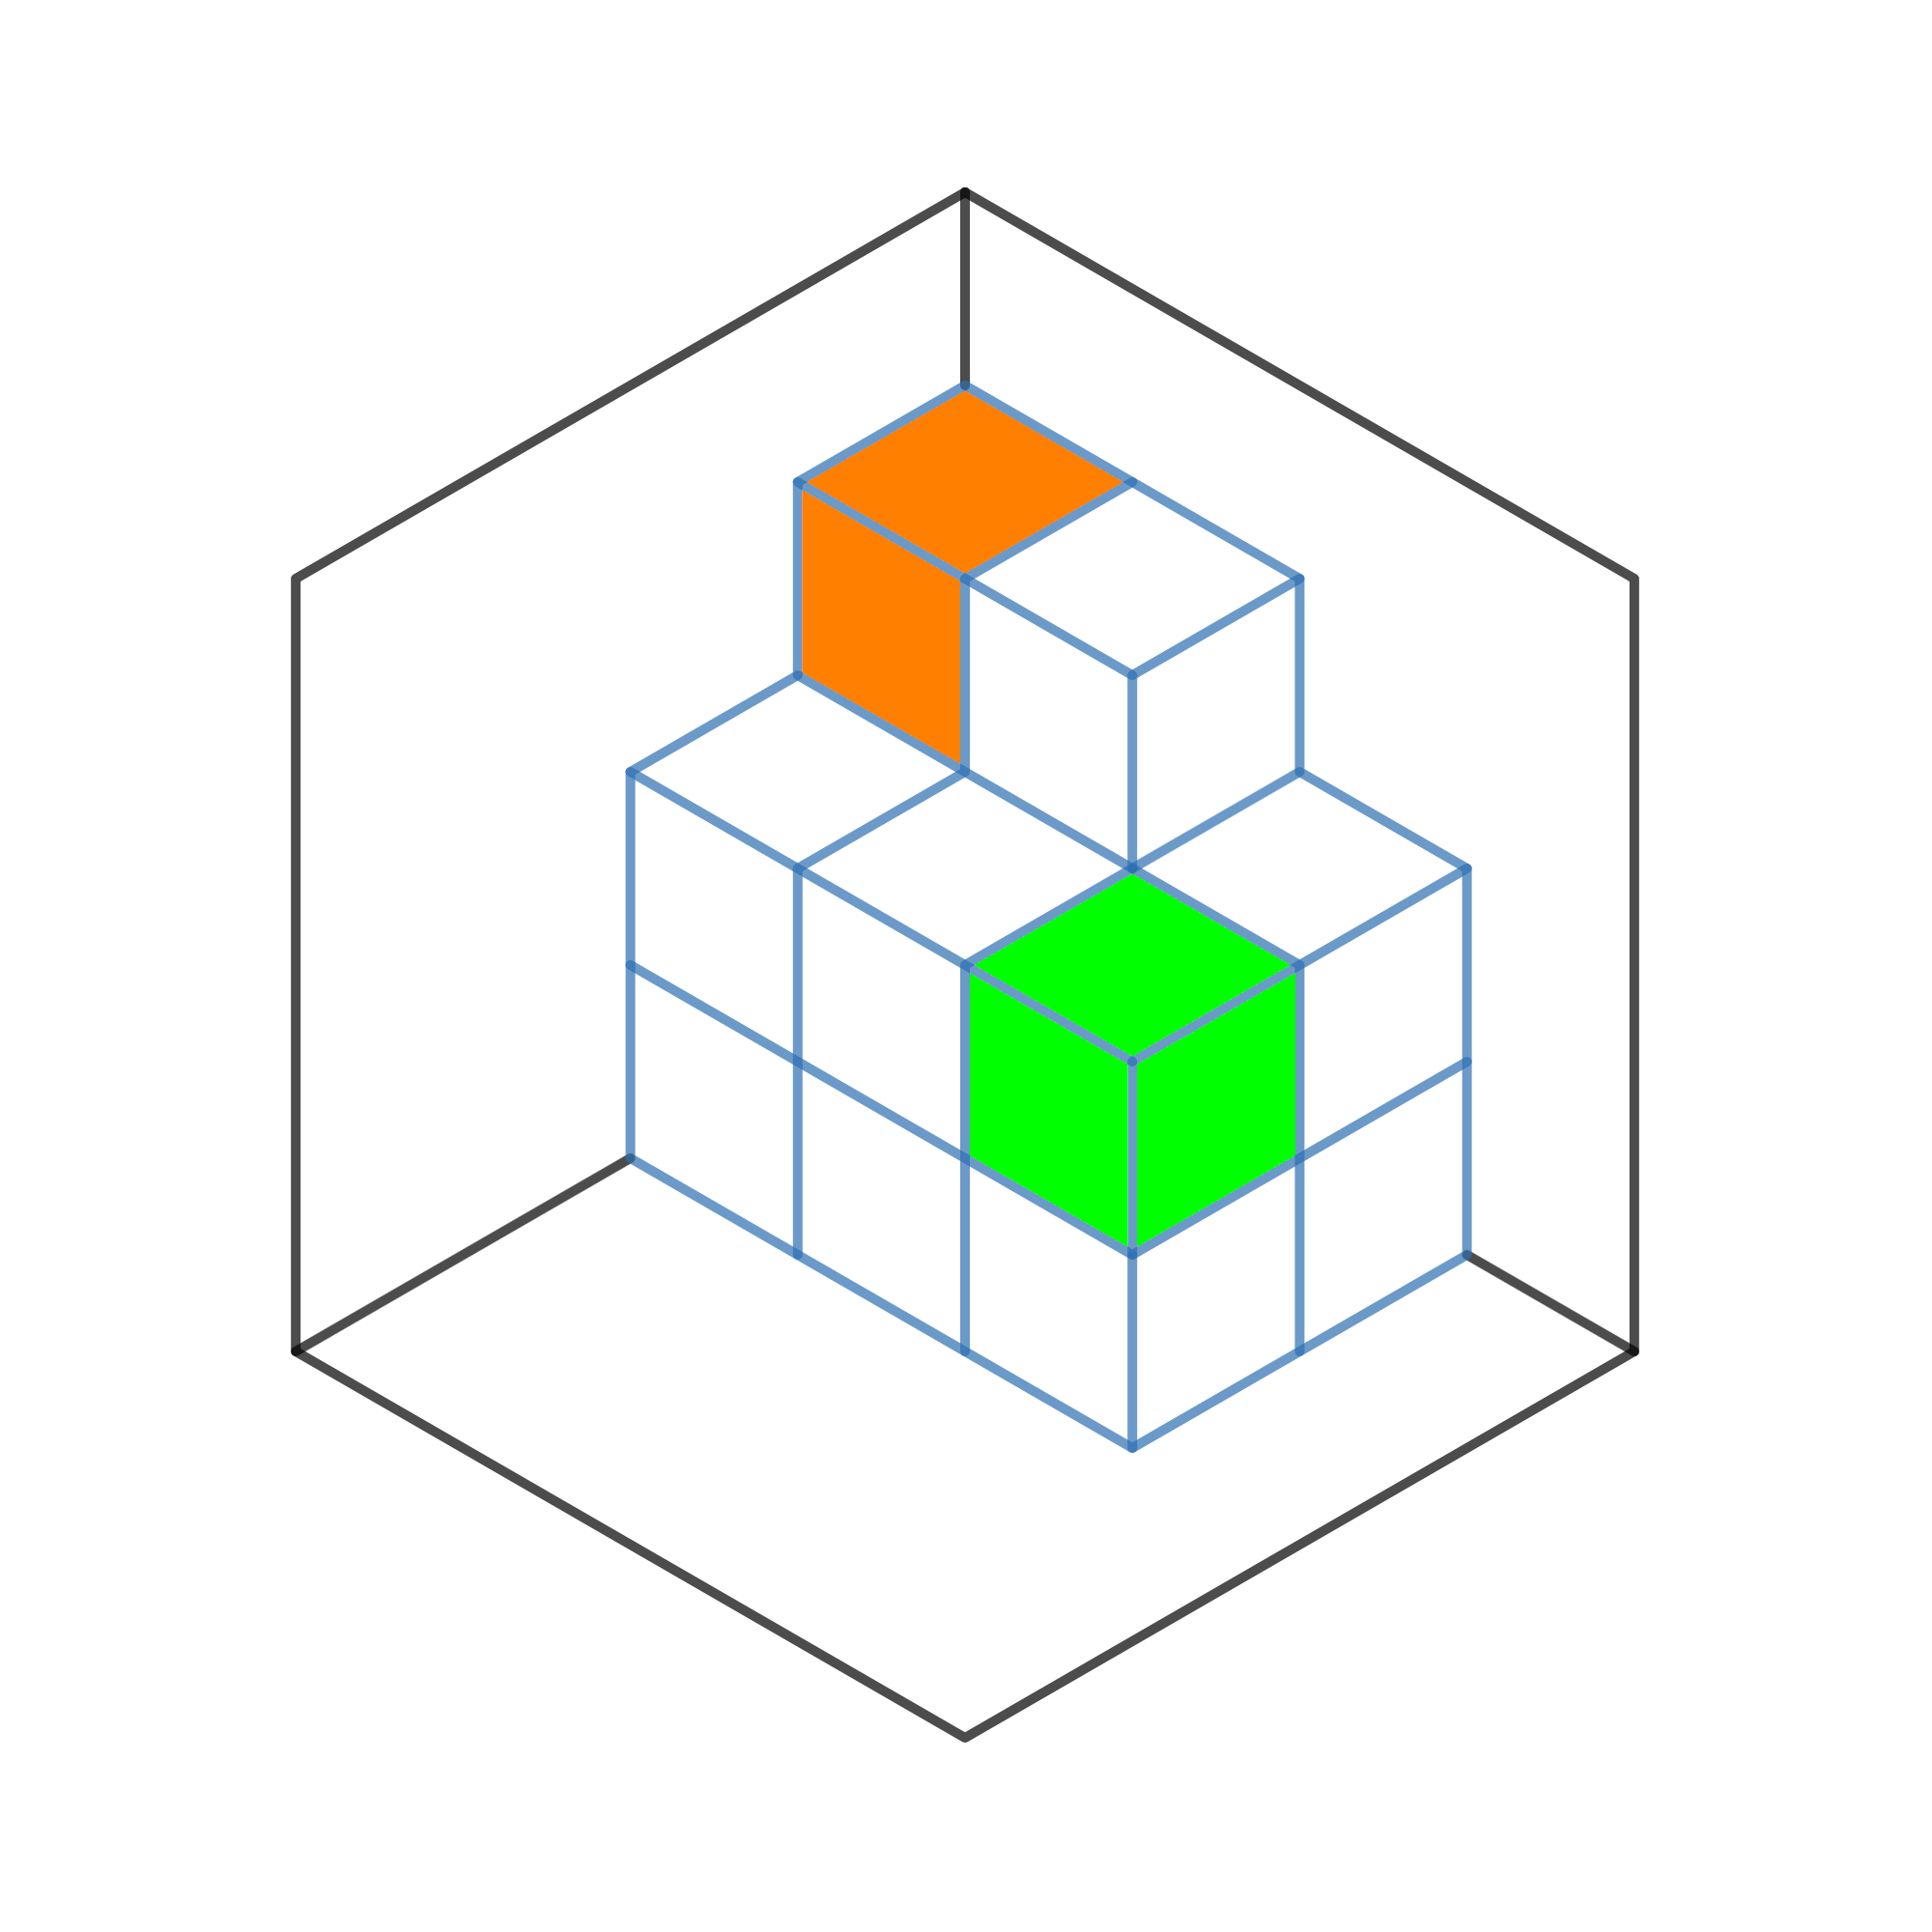
\includegraphics[width=.3\linewidth]{box-stacking}

		

	\end{center}

	
\end{Example}






\end{document}
